%!TEX root = ../dokumentation.tex

\chapter{Darstellung und Interaktion}
Der wichtigste Aspekt bei der Darstellung, ist offensichtlich das Tableau. Da mit diesem vom Benutzer Interagiert werden soll, muss es manuell gezeichnet werden. Deshalb ist der erste Schritt in diesem Kapitel, die Wahl eines geeigneten \ac{GUI} Frameworks, mit dem ein interaktives Tableaux umgesetzt werden kann. Im nächsten Schritt werden verschiedene Darstellungs- und Interaktionskonzepte erarbeitet und verglichen. Der letzte Teil beschreibt die Implementierung des erarbeiteten Konzepts.

\section{Frameworks}
Grundsätzlich gibt es sehr viele \ac{GUI}-Frameworks für Python. Wie zum Beispiel im Falle von PyJamas, ist dies allerdings eher ein JavaScript Konverter mit dem Python Code mit dem Browser als \ac{GUI} laufen kann.

Deshalb fallen bereits schon einige Frameworks aus unserer Betrachtung heraus. Ebenfalls inpraktikabel sind Plattformgebundene Frameworks wie Beispielsweise PyObjC welches nur auf der MacOS Plattform funktioniert.

In dieser Betrachtung werden deshalb nur ein paar bekanntere Frameworks betrachtet. Diese sind:
\begin{itemize}
\item \textbf{TkInter}: Das ``Standard'' Framework welches in der CPython-Distribution mitgeliefert wird.

\item \textbf{PySide2}: Python Bindings für das bekannte C++-Framework \textit{Qt}.

\item \textbf{PyGObject}: Python Bindings für das GTK-Framework.
\end{itemize}
Neben diesen gibt es noch viele weitere Frameworks wobei diese oft Bindings für selbe Frameworks wie Beispielsweise \textit{Qt} sind.

\subsection{TkInter}
Das Framework TkInter hat den Vorteil, als die Standardbibliothek ohne Aufwand direkt verwendet werden zu können. Zudem ist es relativ einfach möglich auf einer Zeichenfläche Linien zu zeichnen und auf selbiger zusätzlich Buttons unterzubringen wie in \autoref{lst:tkinterDrawLine} dargestellt ist.
\begin{lstlisting}[caption={Zeichnen von Linien und Buttons mit TkInter},label=lst:tkinterDrawLine]
import tkinter
class Window(tkinter.Frame):
	...
	def draw_line(self, from, to):
		"""Draws a line on the canvas from 'from' to 'to'"""
		self.canvas.create_line(from.x, from.y, to.x, to.y)
	
	def add_button(self, pos, title, command):
		"""Adds a new button on position with the given title and command callback"""
		new_button = tkinter.Button(self)
		new_button["text"] = title
		new_button["command"] = command
		new_button.place(x=pos.x, y=pos.y)
\end{lstlisting}

Nachteilig ist allerdings, dass es zu diesem Framework keinen moderneren \ac{GUI}-Builder, also eine Software mit der die Benutzeroberfläche graphisch erstellt werden kann, gibt. Die \ac{GUI} muss also im Code erstellt werden. Zudem haben die Standardelemente des Frameworks einen eher veraltetes Aussehen wie in \autoref{fig:screenshot_tkinter} zu sehen ist.

\begin{figure}[h]
\begin{center}
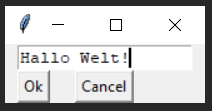
\includegraphics[scale=0.7]{images/tkinter_screenshot.png}
\caption{Screenshot einer mit TkInter erzeugten GUI.}
\label{fig:screenshot_tkinter}
\end{center}
\end{figure}

\subsection{PySide2}
PySide2 ist der Nachfolger von PySide. Das PySide-Framework bietet die Möglichkeit über Python das \textit{Qt-Framework} zu verwenden. \textit{Qt} ist ein Umfangreiches Framework das neben der \ac{GUI} erstellung auch noch weitere Funktionen wie Beispielsweise Datenbankzugriffe ermöglicht.

Das zeichnen von Linien und Buttons in diesem Framework ist ebenfalls relativ einfach wie \autoref{lst:pyside2DrawLine} zeigt. Im Gegensatz zu TkInter muss das zeichnen aber immer in einem paint-event ausgeführt werden.
\begin{lstlisting}[caption={Zeichnen von Linien mit Qt},label=lst:pyside2DrawLine]
class DrawingCanvas(QWidget):
	lines = []
	
	...

	def paintEvent(self, paintEvent):
    	p = QPainter()
    	p.begin(self)
    	for line in lines:
	    	p.drawLine(line)
    	p.end()
\end{lstlisting}
Für \textit{Qt} Anwendungen gibt es zudem einen modernen \ac{GUI}-Builder \textit{Qt Creator}. Die Standardelemente haben wie in \autoref{fig:screenshot_pyside2} dargestellt, auch ein moderneres Aussehen.

\begin{figure}[h]
\begin{center}
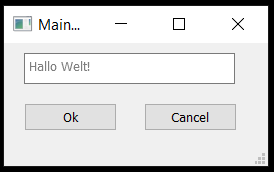
\includegraphics[scale=0.7]{images/pyside2_screenshot.png}
\caption{Screenshot einer mit Qt erzeugten GUI.}
\label{fig:screenshot_pyside2}
\end{center}
\end{figure}

Im Gegensatz zu TkInter muss PySide2 aber über den Paketmanager \textit{pip} nachgeladen werden. Der Aufwand hierfür ist aber vernachlässigbar gering.

\subsection{PyGObject}
Das letzte Framework in dieser Betrachtung ist PyGObject. Mit diesem kann das relativ bekannte Framework Gtk, welches in Anwendungen wie GIMP verwendet wird, in Python verwendet werden.

Vorrausgesetzt die von Gtk unabhängige Bibliothek Cairo ist vorhanden, stellt sich das Zeichnen ebenfalls relativ leicht dar. Dies wird in \autoref{lst:pygobjectDrawLine} dargestellt.
\begin{lstlisting}[caption={Zeichnen von Linien mit Gtk},label=lst:pygobjectDrawLine]
lines = []

def draw(da, ctx):
	ctx.set_source_rgb(0,0,0)
	ctx.set_line_width(1)
	for line in lines:
		ctx.move_to(line.from.x, line.from.y)
		ctx.rel_line_to(line.to.x, line.to.y)
\end{lstlisting}
Ähnlich wie \textit{Qt}, ist auch bei Gtk das zeichnen nur in einem paint-event möglich.

Auch für PyGObject gibt es einen modernen \ac{GUI}-Builder \textit{Glade}. Zudem haben die Standardelemente ebenfalls ein modernes Aussehen wie in \autoref{fig:screenshot_pygobject} zu sehen.

\begin{figure}[h]
\begin{center}
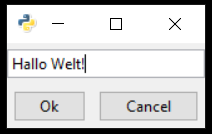
\includegraphics[scale=0.7]{images/pygobject_screenshot.png}
\caption{Screenshot einer mit Gtk erzeugten GUI.}
\label{fig:screenshot_pygobject}
\end{center}
\end{figure}

Die Installation stellt sich hingegen für PyGObject etwas schwieriger dar. Während PySide2 einfach über den Paketmanager geladen werden kann, hat PyGObject noch weitere externe Abhängigkeiten die aufwändig hinzu installiert werden müssen.

\subsection{Gesamtübersicht}
Eine Gesamtübersicht der betrachteten Faktoren bei den Frameworks wird in \autoref{tbl:comparison_gui_frameworks} dargestellt.
\begin{table}[h]
\begin{center}
\begin{tabular}{c|c|c|c|c}
Framework & Einfachheit & Aussehen & GUI-Builder & Installation \\
\hline
TkInter & {\cellcolor{green!50}}Sehr einfach & \cellcolor{red!50}Veraltet & \cellcolor{red!50}Schlecht & \cellcolor{green!50}Bereits installiert \\
Qt & \cellcolor{green!25}Einfach & \cellcolor{green!50}Modern & \cellcolor{green!50}Gut & \cellcolor{green!25}Leicht über Paketmanager \\
Gtk & \cellcolor{green!25}Einfach & \cellcolor{green!50}Modern & \cellcolor{green!50}Gut & \cellcolor{red!50}Schwierig
\end{tabular}
\end{center}
\caption{\label{tbl:comparison_gui_frameworks}Gesamtübersicht der 3 verglichenen GUI-Frameworks}
\end{table}

Das einzige Framework ohne größere Defizite ist also \textit{Qt}, weshalb dieses verwendet wird.

\section{Konzepterarbeitung}
Prinzipiell gibt es an die \ac{GUI} folgende Anforderungen:
\begin{itemize}
\item \textbf{Leichte Übersicht über Tableau}: Das Gesamte Tableau anzusehen soll auch bei großen Tableaux möglichst einfach realisierbar sein.

\item \textbf{Benutzerfreundliche Interaktion}: Beim Interaktiven Modus soll der Benutzer die einzelnen Ableitungsschritte selbst eingeben und Feedback über Korrektheit bekommen. Dies soll Benutzerfreundlich möglich sein.

\item \textbf{Einfaches umschalten zwischen Modi und Logik}: Der Tableaux-Beweiser soll in zwei verschiedenen Modi laufen: Automatisch oder Interaktiv. Zudem kann zwischen 4 Logiken (klassische/nichtklassische Aussagenlogik/Prädikatenlogik) umgeschalten werden. Die Umschaltung zwischen den Modi und Logiken sollte einfach sein.

\item \textbf{Hilfebeschreibungen}: Über verschiedene Eigenheiten (z.B. welches Zeichen für die Negation verwendet wird) soll in der \ac{GUI} aufgeklärt werden. Auch die Allgemeine Bedienung muss Intuitiv möglich bzw. in einer Hilfe beschrieben sein.

\item \textbf{}
\end{itemize}

Aufgrund dieser Anforderungen werden nachfolgend verschiedene Konzepte erarbeitet und verglichen.

\subsection{Konzept 1}
Für das erste Konzept werden 2 Fenster für die Hauptinteraktion benötigt. Das erste Fenster (Hauptfenster), stellt das gesamte Tableau dar. Im Hauptfenster kann zudem zwischen den Modi Automatik und Manuell gewechselt werden. Im Modus Automatik, ist nach dem Start der automatischen Ableitung keine weitere Interaktion nötig/möglich außer dem Start einer neuen Ableitung. Der erste Entwurf des Konzepts im Automatikbetrieb, ist in \autoref{fig:gui_concept_1_automatic} zu sehen.

\begin{figure}[h]
\begin{center}
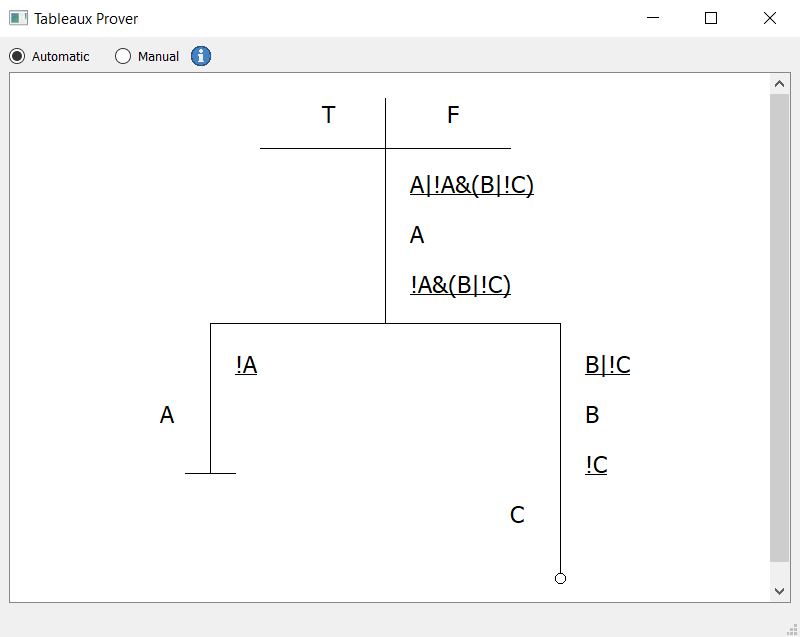
\includegraphics[scale=0.7]{images/gui_concept_1_automatic.png}
\caption{Konzept 1 im Modus Automatik}
\label{fig:gui_concept_1_automatic}
\end{center}
\end{figure}

Im Modus Manuell, muss jeder Ableitungsschritt vom Benutzer selbst ausgeführt werden. Hierfür wird jede noch nicht verarbeitete, nicht Atomare Formel als Button dargestellt. Dies ist in \autoref{fig:gui_concept_1_manual} zu sehen.

\begin{figure}[h]
\begin{center}
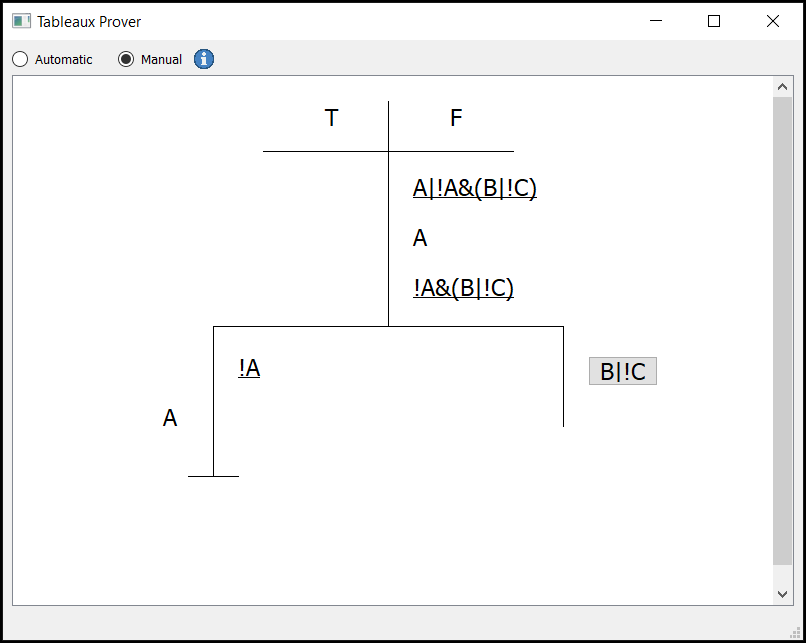
\includegraphics[scale=0.7]{images/gui_concept_1_manual.png}
\caption{Konzept 1 im Modus Manuell}
\label{fig:gui_concept_1_manual}
\end{center}
\end{figure}

Wird ein solcher Formel-Button betätigt, öffnet sich das zweite Fenster (Ableitungseingabefenster). Im Ableitungseingabefenster kann ausgewählt werden ob die Ableitung der Formel eine verzweigte oder nicht verzweigte ist. Die Eingabe einer nicht verzweigten Ableitung, nach Betätigung des Buttons \enquote{B|!C} (B$\vee\neg$C, siehe Syntaxdefinition \textbf{EINGEBEN!!!!!}) zeigt \autoref{fig:gui_concept_1_manual_enter_single}.

\begin{figure}[h]
\begin{center}
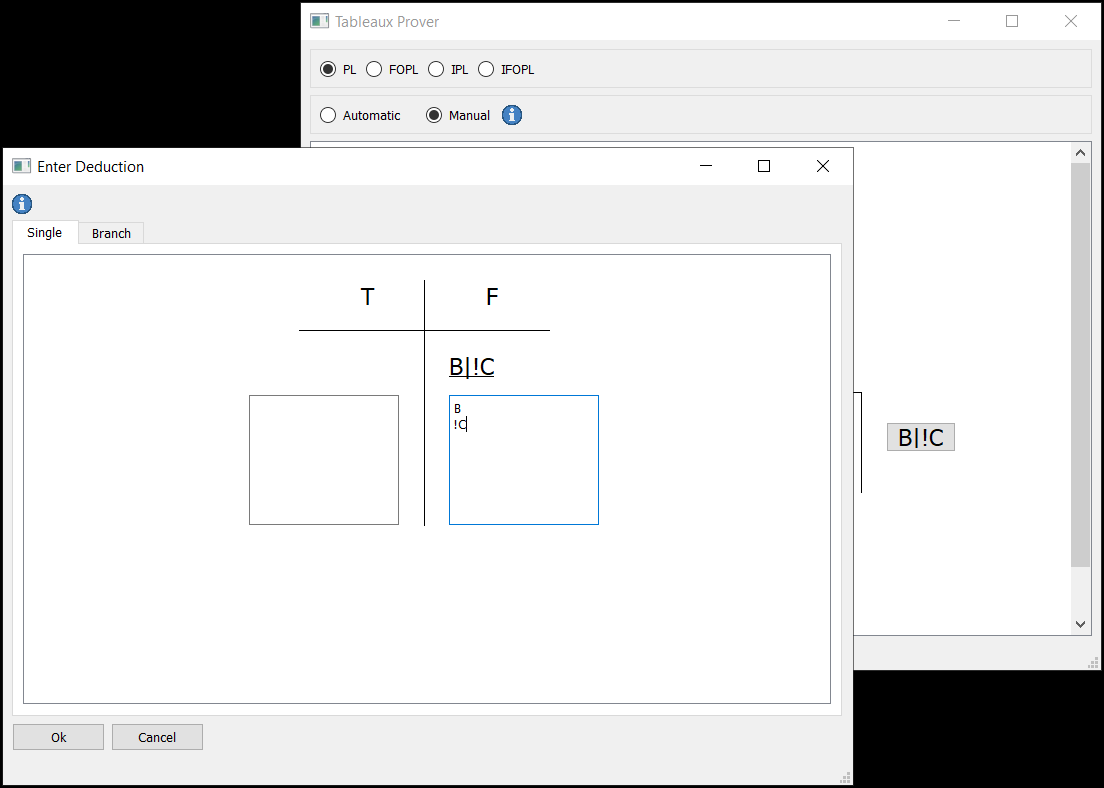
\includegraphics[scale=0.7]{images/gui_concept_1_manual_enter_single.png}
\caption{Konzept 1: Eingabe einer Ableitung im Modus Manuell}
\label{fig:gui_concept_1_manual_enter_single}
\end{center}
\end{figure}

Die Eingabe einer verzweigenden Ableitung, nach Betätigen des Buttons \enquote{B\&!C} (B$\wedge\neg$C siehe Syntaxdefinition \textbf{EINGEBEN!!!!}) zeigt \autoref{fig:gui_concept_1_manual_enter_branch}.

\begin{figure}[h]
\begin{center}
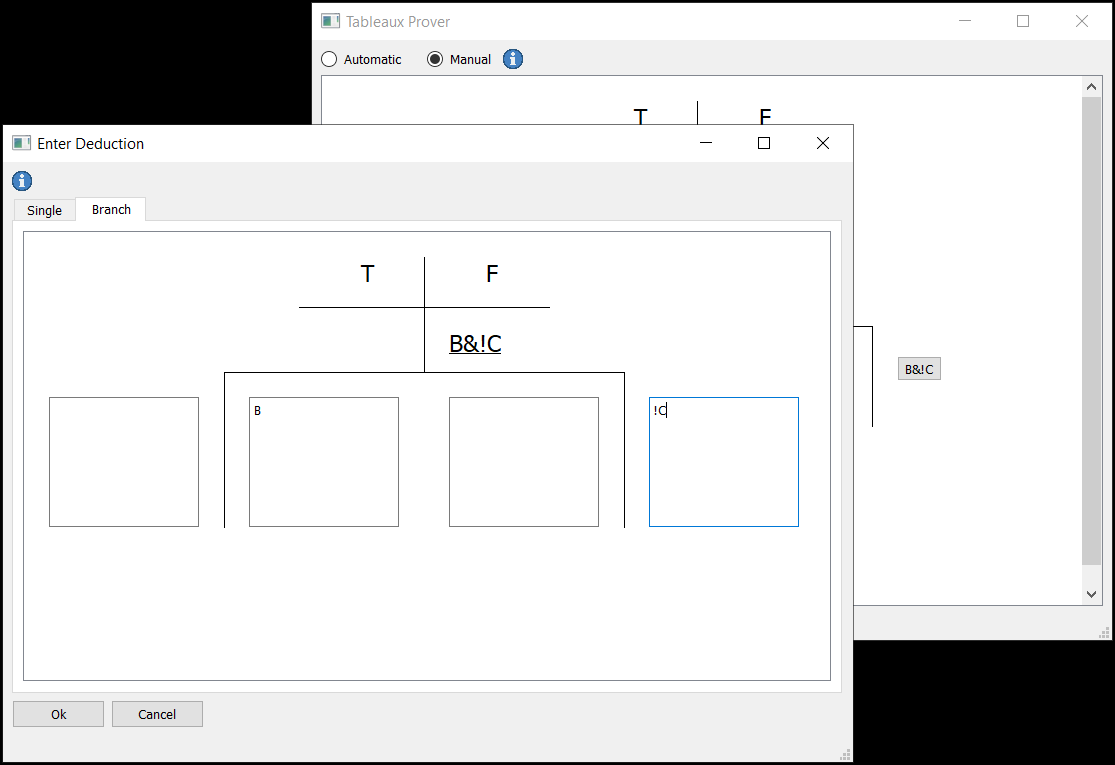
\includegraphics[scale=0.7]{images/gui_concept_1_manual_enter_branch.png}
\caption{Konzept 1: Eingabe einer verzweigenden Ableitung im Modus Manuell}
\label{fig:gui_concept_1_manual_enter_branch}
\end{center}
\end{figure}

\subsection{Konzept 2}
Das zweite Konzept ähnelt dem ersten stark. Der Unterschied hierbei ist, es muss keine Formel zur Ableitung ausgewählt werden sondern nur das Ergebnis eingegeben werden. Im Modus Automatik ist die Funktionsweise die selbe wie bei Konzept 1, siehe \autoref{fig:gui_concept_1_automatic}.

Im Modus Manuell hingegen, kann an das Tableau an den noch nicht geschlossenen Zweigen erweitert werden. Hierbei gibt es zwei Möglichkeiten, bei einer nicht verzweigenden Ableitung wird das Ergebnis in die Textfelder eingegeben und der +-Button betätigt. Dies ist in \autoref{fig:gui_concept_2_manual_enter_single} zu sehen.
\begin{figure}[h]
\begin{center}
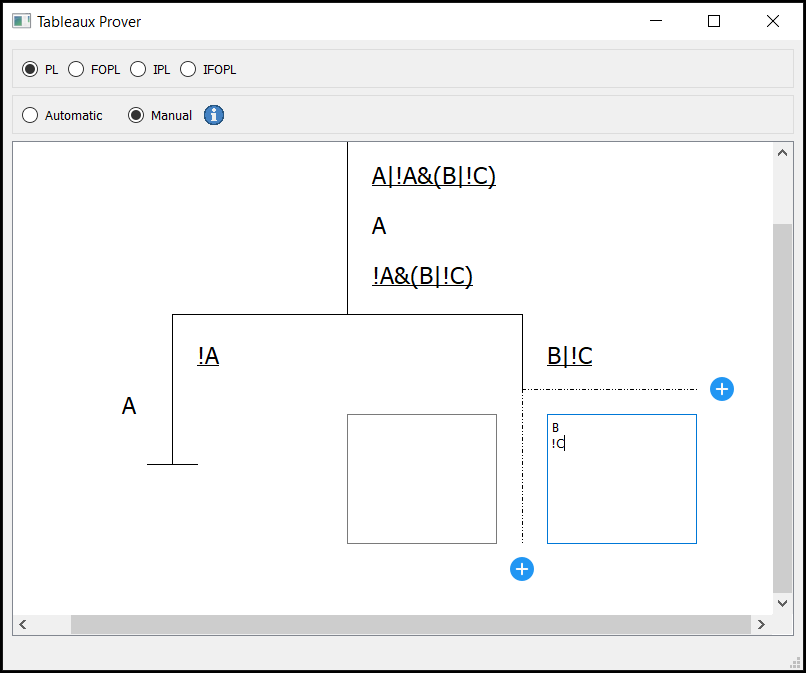
\includegraphics[scale=0.7]{images/gui_concept_2_manual_enter_single.png}
\caption{Konzept 2: Eingabe einer Ableitung im Modus Manuell}
\label{fig:gui_concept_2_manual_enter_single}
\end{center}
\end{figure}

Wird hingegen eine verzweigende Ableitung behandelt, kann ein neuer Zweig über den nach Rechts angedeuteten Pfad mit dem +-Button geöffnet werden. Die Eingabe der Ableitung erfolgt dann ebenfalls in den Textfeldern und wird über die +-Buttons bestätigt. Dies wird in \autoref{fig:gui_concept_2_manual_enter_branch} dargestellt.

\begin{figure}[h]
\begin{center}
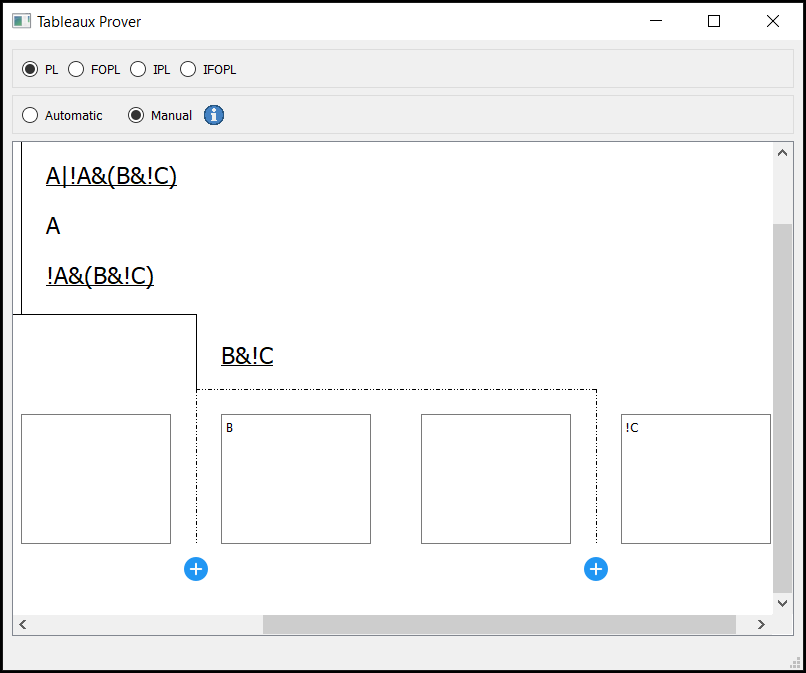
\includegraphics[scale=0.7]{images/gui_concept_2_manual_enter_branch.png}
\caption{Konzept 2: Eingabe einer verzweigenden Ableitung im Modus Manuell}
\label{fig:gui_concept_2_manual_enter_branch}
\end{center}
\end{figure}

Die Behandlung einer nur Teilweise eingegebenen verzweigenden Ableitung erhöht dabei die Komplexität des Konzepts erheblich. Problematisch ist aber vor allem die Unübersichtlichkeit, wird in einem großen Tableau eine weit oben stehende Formel abgeleitet. Zudem muss eine verzweigende Ableitung in jedem der nachfolgenden Zweige erneut eingegeben werden was die Benutzerfreundlichkeit einschränkt und die Implementierung erschwert.

\section{Konzept 3}

